\documentclass[french,a4paper,10pt]{article}

\usepackage[a4paper,hmargin=30mm,vmargin=30mm]{geometry}
\usepackage[T1]{fontenc} % font type
\usepackage[french]{babel} % language
\usepackage{lmodern} % font type
\usepackage[shortlabels]{enumitem}
\usepackage{hyperref}
\usepackage{graphicx}
\usepackage{sectsty}
%\setlength{\parindent}{0pt}



\title{Compte Rendu TP2\\Opérations morphologies sur des images}
\author{Ivan Lejeune}
\date{\today}


\begin{document}

	\maketitle

	% make table of contents
	\tableofcontents

	\newpage
	\section{Seuillage d'une image et erosion de l'image binaire}\label{sec:1}

	\subsection{Choix de l'image}

	On commence par choisir une image, dans notre cas on a choisi l'image \texttt{08.pgm}, et ensuite on la reduit pour
	qu'elle soit de taille 256x256. Cela donne alors :
	% insert side by side original image vs reduced image

	\begin{figure}[!htb]
		\begin{minipage}{0.48\textwidth}
			\centering
			\fbox{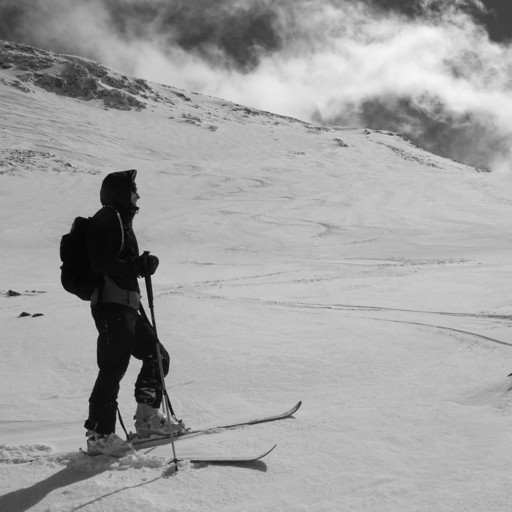
\includegraphics[width=.7\linewidth]{./out/orig-08}}
			\caption{Image originale}\label{Fig:orig-08}
		\end{minipage}\hfill
		\begin{minipage}{0.48\textwidth}
			\centering
			\fbox{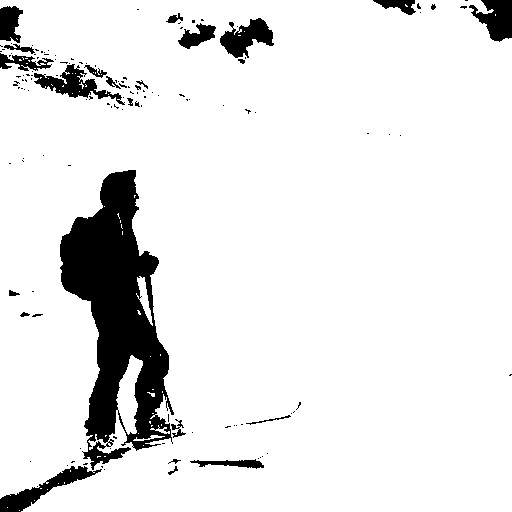
\includegraphics[width=.7\linewidth]{./out/test-grey-08}}
			\caption{Image modifiée avec un seuil de 80}\label{Fig:test-grey-08}
		\end{minipage}
	\end{figure}
\end{document}
